\begin{figure*}[t]
    \begin{subfigure}[b]{\linewidth}
        \centering
        % trim={<left> <lower> <right> <upper>}
        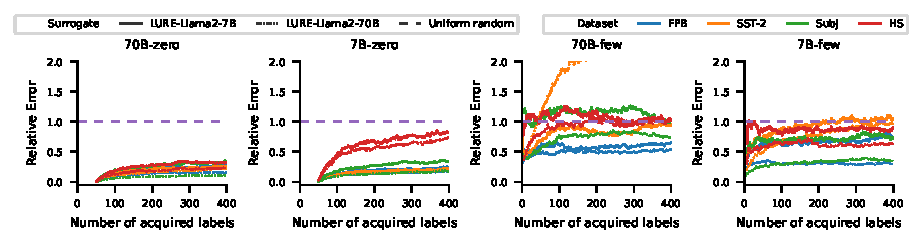
\includegraphics[width=\linewidth,trim={8pt 5pt 0 0}]{
            figures/pdf/70b_7b_zeroshot_fewshot_relative_error.pdf
        }
        \caption{Llama 2 target models and Llama 2 surrogate models}
         \label{fig:7b_70b_llama_unif_lure}
    \end{subfigure}
    \begin{subfigure}[b]{\linewidth}
        \centering
        % trim={<left> <lower> <right> <upper>}
        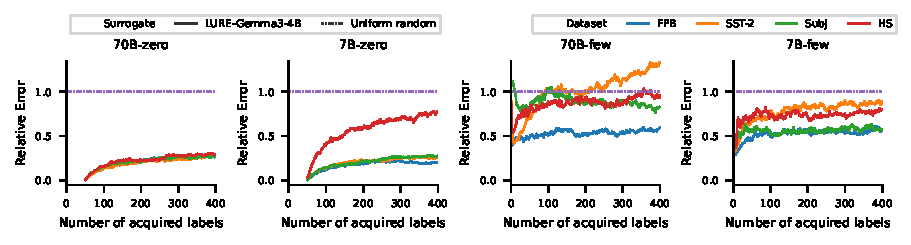
\includegraphics[width=\linewidth, trim={5pt 5pt 0 0}]{
            figures/pdf/relative_errors_gemma.pdf
        }
        \caption{Llama 2 target models and Gemma3-4B surrogate model}
        \label{fig:7b_70b_gemma_unif_lure}
    \end{subfigure}
    \caption{
        Cheap surrogate models support effective data acquisition for active testing.
        We compare uniform-random testing to active testing (LURE) across four datasets.
        To guide active data acquisition we use a surrogate model that we train using a single step of in-context learning and then keep fixed.
        This stripped-back surrogate-model training, along with the use of small surrogate models relative to the target models, allows us to drastically reduce the computational cost of active testing while achieving strong performance.
    }
    \label{fig:7b_70b_zeroshot_fewshot_unif_lure}
    \vspace{-8pt}
\end{figure*}